\documentclass[12pt,fleqn]{article}\usepackage{../../common}
\begin{document}
Sıvı Dinamiğinde Sonlu Hacim Metotu - 1

Ağırlıklı Artıklar Metotu (Weighted Residual Method -WRM-)

Önceki derste iyi koşullu bir sistemi elde etmeyi gördük, bu kötü koşullu (ill
conditioned) olmanın tersi tabii. Bu derste [1] WRM'yi kurmayı göreceğiz, ki bu
metot aslında kapsayıcı bir tarif, altında farklı hesap yöntemleri de
olabiliyor, WRM'nin kendisi hata kontrolünü nasıl yapacağımızı tarif ediyor.

Basit bir problemle başlayalım. Laplace formülü mesela, iki boyutu baz alalım,
ama birazdan göreceğimiz fikirler 1D ya da 3D için de geçerli. Problem bölgesi
(domain) $\Omega$ olsun onun sınırları $\Gamma$, 

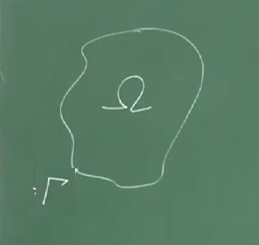
\includegraphics[width=15em]{compscieng_app45aerofem1_01.png}

İlgilendiğimiz alan (field) $T(x,y)$, bu reel değerli bir fonksiyon, ve
kurduğumuz sistem için bu fonksiyonun şu şartlara tabi olmasını istiyoruz,

$$
\nabla^2 T = 0 \quad \Omega \textrm{ üzerinde } 
$$

$$
\Gamma \textrm{ için } T = T_0
$$

Bu tur problemlere Drichlet problemleri deniyor.

Üstteki şartları yerine getiren bir $T(x,y)$ çözümü bulmak istiyoruz. O zaman
ilk akla gelen nedir? Diferansiyel denklemi alıyorum ve $\Omega$ içindeki tüm
noktalar için çözmeye uğraşıyorum. Fakat bu kolay değil. Ayrıca $\Omega$'daki
eşitlik $\Gamma$ sınırında geçerli değil, ikinci şart sebebiyle. Bu arada
matematiksel olarak çözüm nedir? $\Omega$'daki sonsuz tane nokta için geçerli
olan şeydir. Buna kesin çözüm (exact solution) deniyor. 

Fakat bu çözümü bulmak mümkün değilse, ya da yaklaşık bir çözüm de yeterli
oluyorsa o zaman yaklaşık yöntemler kullanabilirim.. $\nabla^2 T = 0 $ eşitliği
$\Omega$'daki her nokta için, her $\Gamma$ sınır şartında değil belli seçilmiş
noktalarda olsun diyebilirim.

Ama ``belli noktalarda'' deyince de iş bitmiyor, o seçilmiş noktalarda kesin
çözüm mü yapsam, yoksa o noktalarda da yaklaşık çözüm yapsam? Ya da tüm
noktalarda yaklaşık çözüm üzerinden bir hata hesaplayıp, tüm seçilmiş noktalarla
hesaplanan ortalama bir hatanın sıfır olması için mi uğraşsam?

Şöyle bir yöntem deneyelim; elimizde / verili belli bir baz fonksiyon ``sınıfı''
olsun, bu fonksiyonlar Fourier bazı $\sin$, $\cos$ olabilir, ya da Chebisev
polinomları olabilir. Bu ``test'', baz fonksiyonları $T_i(x,y)$ içinde,
$i=1,2,...,N$, ve nihai $T$'yi

$$
T = T_0 + \sum _{i=1}^{N} c_i T_i(x,y)
$$

ile hesaplayayım, $c_i$'ler başta bilmediğim katsayı değerleri olsun. Bilinen /
verili test fonksiyonları üzerinden doğru $c_i$'leri bulursam bu beni gerçek
fonksiyon $T$'ye yaklaştırır. Üstteki toplamda $T_0$ terimi özellikle o şekilde
formüle dahil edildi, $T_i$ toplamının sınırda sıfır olmasını ayarlayabilirsem,
$T=T_0$ şartını otomatik olarak tatmin etmiş olurum.

$N$ sayısına dikkat, gerçek fonksiyonu aşağı yukarı temsil etmek istesem $N$'yi
az tutardım, birkaç tane temel fonksiyon birleşimi.. Ama $N$'i arttırarak, hatta
sonsuza yaklaştığımızda gerçek fonksiyona tıpatıp eşit olacağımızı
bekleyebilirdik, o zaman $N$ sayısı bir anlamda yaklaşıklamanın kalitesini
kontrol edecektir. $N$ arttıkça hata azalır, yaklaşıklama gerçeğe yaklaşır.
Bir ödünleşim (trade-off) durumu var muhakkak, çok büyük $N$ hesaplaması zor
olan bir sistem ortaya çıkartabilir, vs.

Bu bizi hata tanımına getiriyor. Onu gerçek ve yaklaşık değerler arasındaki
fark, ``artık'' (residual) üzerinden tanımlayacağız, artık $R$,

$$
R(c_i,x,y) = \nabla^2 T
$$

Bu kadar basit. Niye artığı direk $\nabla^2 T$'e eşitlemek yeterli? Çünkü ana
formüle bakarsak $\nabla^2 T$ ideal durumda sıfır olmalı değil mi?  Ama
yaklaşıklama mükemmel olmadığı için sıfırdan farklı (fakat umuyoruz ki ona
yakın) değerler döndürecektir, o zaman bu değeri alıp direk hata / artık değeri
olarak kullanabiliriz. O zaman

$$
R(c_i,x,y) = T_0 + \sum _{i=1}^{N} c_i T_i(x,y)
$$

diyelim. Üstteki denklem bana her veri noktası, belli bir $x,y$ için olan hatayı
verir. Sınır koşulunu denklem doğal olarak karşıladığı için orada zaten hata
yok. Yani tanım itibariyle sınırda hata sıfır, ve sınırlar içinde muhtemel
olarak sıfır olmayan bir değerde.

Şimdi $c_i$'lerin bulunmasına gelelim, yaklaşık temsil onlar üzerinden mümkün
olacak. $N$ tane $c_i$ bilinmiyor o zaman bir şekilde $N$ tane denklem üretmem
lazım, ki onları çözerek bilinmeyenleri elde edeyim. WRM burada devreye giriyor.

Agirlikli artiklar dedik, agirliklardan da (dikkat $c_i$ katsayilarindan, ve
test fonksiyonlarindan farkli bu) da $N$ tane var, $N$ tane fonksiyon. Onlari
$j$ ile indisleyebiliriz, $w_j$, $j=1,...,N$. Artiklari soyle agirlikliyoruz,

$$
\int_\Omega w_j R \ud \Omega
$$

Biraz önce söylediğimiz artığın sıfır olma hedefini biraz genişletip
ağırlıklanmış artığın sıfır olması haline getiriyoruz. O zaman $N$ tane denklemi
şöyle üretiriz,

$$
j=1,\quad
\int_\Omega w_1 (x,y) \left[
  \nabla^2 T_0 + \sum _{i=1}^{N} c_i \nabla^2 T_i(x,y) 
  \right] \ud \Omega
$$

$$
j=2,\quad
\int_\Omega w_2 (x,y) \left[
  \nabla^2 T_0 + \sum _{i=1}^{N} c_i \nabla^2 T_i(x,y) 
  \right] \ud \Omega
$$

$$
\vdots
$$

$$
j=N,\quad
\int_\Omega w_N (x,y) \left[
  \nabla^2 T_0 + \sum _{i=1}^{N} c_i \nabla^2 T_i(x,y) 
  \right] \ud \Omega
$$

Böylece $N$ tane bilinmeyen için $N$ tane formül elde ettim, ve bu şekilde
çözümü yapabilirim.

$w_j$'ler ne yapıyor? Başta hataların ortalamasından bahsetmiştik hatırlarsak,
her $w_j$ bir nevi ortalamadır, ama her $j$ icin farkli bir ortalama sekli
secebiliriz, mesela alttaki resimde

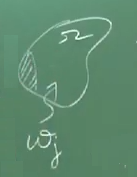
\includegraphics[width=10em]{compscieng_app45aerofem1_02.png}

karalanmış kısma daha fazla ağırlık ver diyebiliriz, vs. Genel anlamda
hatırlarsak mesela üç sayı A,B,C ortalaması demek aslında her sayının 1/3
``ağırlığı'' ile çarpılıp, toplanması ve sonucun 3'e bölünmesi demektir. Bu
ağırlıkları değiştirebiliriz, o zaman farklı bir ortalama elde ederiz, mesela
1/2, 1/4, 1/4 kullansam A'ya daha fazla ağırlık vermiş olurdum.



[devam edecek]

Kaynaklar

[1] Mittal, {\em FEM for Fluid Dynamics, Lecture07 PartA, Method of Weighted Residuals, IIT Kanpur},
    \url{https://www.youtube.com/channel/UCWheqBdP45xBVp_Eqi1eltQ/videos}

\end{document}


